	\documentclass{libs/ufc_format}
\usepackage{amsmath, tikz, graphicx}
\usetikzlibrary{trees,shapes, calc, external, fit, arrows,decorations,decorations.pathreplacing,patterns, automata, positioning, arrows.meta}

\newcommand{\starpu}{\textsc{StarPU}\xspace}
\newcommand{\GPU}[1]{\ensuremath{\mathrm{GPU}_{#1}}\xspace}
\newcommand{\Node}[1]{\ensuremath{\mathrm{Node}_{#1}}\xspace}
\newcommand{\flow}[1]{\ensuremath{\mathit{flow}_{#1}}\xspace}
\newcommand{\inputs}{\ensuremath{\mathcal{F}}\xspace}
\newcommand{\memory}{\ensuremath{\mathcal{M}}\xspace}
\newcommand{\memorymap}{\ensuremath{\mathcal{M}_{map}}\xspace}
\newcommand{\duration}{\mathit{Duration}\xspace}
\newcommand{\bandwidth}{\mathit{BW}\xspace}
\newcommand{\core}{\mathit{Cores}\xspace}
\newcommand{\submissiontime}{\mathit{Subtime}\xspace}
\newcommand{\walltime}{\mathit{Walltime}\xspace}
\newcommand{\completiontime}{\mathit{Completiontime}\xspace}
\newcommand{\start}{\mathit{Starttime}\xspace}
\newcommand{\fileset}{\ensuremath{\mathbb{F}}\xspace}
\newcommand{\jobset}{\ensuremath{\mathbb{J}}\xspace}
\newcommand{\evict}{\ensuremath{\mathcal{V}}\xspace}
\newcommand{\nbloads}{\ensuremath{\mathit{\mathit{Loads}}}\xspace}
\newcommand{\live}{\ensuremath{L}\xspace}
%%%%%%%%%%%%%%%%%%%%%%%%%%%%%%%%%%%%%%%%%%%%%%%%%%%%%%%%%%%%%%%%%%%%%%%%%%%%%%%%%%%

% For the arrows in circle
\setcounter{tocdepth}{1}
\usetikzlibrary{decorations.text}
\newcommand*{\mytextstyle}{\sffamily\small\bfseries\color{black!85}}
\newcommand{\arcarrow}[8]{%
% inner radius, middle radius, outer radius, start angle,
% end angle, tip protusion angle, options, text
  \pgfmathsetmacro{\rin}{#1}
  \pgfmathsetmacro{\rmid}{#2}
  \pgfmathsetmacro{\rout}{#3}
  \pgfmathsetmacro{\astart}{#4}
  \pgfmathsetmacro{\aend}{#5}
  \pgfmathsetmacro{\atip}{#6}
  \fill[#7] (\astart:\rin) arc (\astart:\aend:\rin)
       -- (\aend+\atip:\rmid) -- (\aend:\rout) arc (\aend:\astart:\rout)
       -- (\astart+\atip:\rmid) -- cycle;
  \path[font = \sffamily, decoration = {text along path, text = {|\mytextstyle|#8},
    text align = {align = center}, raise = -0.5ex}, decorate]
    (\astart+\atip:\rmid) arc (\astart+\atip:\aend+\atip:\rmid);
}

\newcommand{\nologo}{\setbeamertemplate{logo}{}} % command to set the logo to nothing

% Inserting the preamble file with the packages
%%%%%%%%%%%%%%%%%%%%%%%%%%%%%%%%%%%%%%%%%%%%%%%%%%%%%%%%%%%%%%%%%%%%%
%% This file contains the packages that can be used in the beamer. %%
%%%%%%%%%%%%%%%%%%%%%%%%%%%%%%%%%%%%%%%%%%%%%%%%%%%%%%%%%%%%%%%%%%%%%
% Package to fonts family
\usepackage[T1]{fontenc}
% Package to accentuation
\usepackage[utf8]{inputenc}
% Package to Portuguese language
\usepackage[english]{babel}
% Package to Figures
\usepackage{graphicx}
% Package to the colors
\usepackage{color}
% Package to the colors
\usepackage{xcolor}
% Packages to math symbols and expressions
\usepackage{amsfonts, amssymb, amsmath}
% Package to multiple lines and columns in table
\usepackage{multirow, array} 
% Package to create pseudo-code
% For more detail of this package: http://linorg.usp.br/CTAN/macros/latex/contrib/algorithm2e/doc/algorithm2e.pdf
\usepackage{algorithm2e}
% Package to insert code
\usepackage{listings} 
\usepackage{keyval}
% Package to justify text
\usepackage[document]{ragged2e}
% Package to manage the bibliography
\usepackage[backend=biber, style=numeric, sorting=none]{biblatex}
% Package to facilities quotations
\usepackage{csquotes}
% Package to use multicols
\usepackage{multicol}
% Subfigures
\usepackage{subcaption}
\usepackage{marvosym} % \MVRIGHTarrow

% Inserting the references file
\bibliography{../ref_cadre.bib}

% Title
\title[Memory-Aware Scheduling]{\huge\textbf{Locality-Aware Batch Scheduling of Jobs Sharing Input Files}}
% Subtitle
\subtitle{Uppmax meeting}
% Author of the presentation
\author{\underline{Maxime GONTHIER} - Loris MARCHAL - Samuel THIBAULT - Elisabeth Larsson - Carl Nettelblad}
% Institute's Name
\institute[UFC]{
    % email for contact
    %~ \normalsize{Loris MARCHAL - Samuel THIBAULT}
    \normalsize{\email{maxime.gonthier@ens-lyon.fr}}
    \newline
    % Department Name
    \department{LIP - ROMA - LaBRI - STORM}
    \newline
    %~ 
\includegraphics[scale=0.05]{Images/solahris+inria.png}%
    % university name
    %~ \univ
}
%~ \titlegraphic{
\includegraphics[scale=0.5]{Images/logo_solharis_full2.png}}

% date of the presentation
% \date{\today}
%~ \usepackage{datetime}
%~ \newdate{date}{01}{06}{2022}
%~ \date{\displaydate{date}}


%%%%%%%%%%%%%%%%%%%%%%%%%%%%%%%%%%%%%%%%%%%%%%%%%%%%%%%%%%%%%%%%%%%%%%%%%%%%%%%%%%
%% Start Document of the Presentation                                           %%               
%%%%%%%%%%%%%%%%%%%%%%%%%%%%%%%%%%%%%%%%%%%%%%%%%%%%%%%%%%%%%%%%%%%%%%%%%%%%%%%%%%
\begin{document}
% insert the code style
%%%%%%%%%%%%%%%%%%%%%%%%%%%%%%%%%%%%%%%%%%%%%%%%%%%%%%%%%%%%%%%%%%%%%%%%%%%%%%%%%%%
%% This file contains the style of the codes show in slides.                     %%
%% The package used is listings, but it possible to used others.                 %%
%%%%%%%%%%%%%%%%%%%%%%%%%%%%%%%%%%%%%%%%%%%%%%%%%%%%%%%%%%%%%%%%%%%%%%%%%%%%%%%%%%%

% color used in the code style
\definecolor{codegreen}{rgb}{0,0.6,0}
\definecolor{codegray}{rgb}{0.5,0.5,0.5}
\definecolor{codepurple}{rgb}{0.58,0,0.82}
\definecolor{codebackground}{rgb}{0.95,0.95,0.92}

% style of the code!
\lstdefinestyle{codestyle}{
    backgroundcolor=\color{codebackground},   
    commentstyle=\color{codegreen},
    keywordstyle=\color{magenta},
    numberstyle=\tiny\color{codegray},
    stringstyle=\color{codepurple},
    basicstyle=\ttfamily\footnotesize,
    frame=single,
    breakatwhitespace=false,         
    breaklines=true,                 
    captionpos=b,                    
    keepspaces=true,                 
    numbers=left,                    
    numbersep=5pt,                  
    showspaces=false,                
    showstringspaces=false,
    showtabs=false,                  
    tabsize=2,
    title=\lstname 
}

\lstset{style=codestyle}


%% ---------------------------------------------------------------------------
\begin{frame}{}
    \maketitle
\end{frame}

%~ %% ---------------------------------------------------------------------------
\begin{frame}{Who am I ?}
	From Bordeaux (France)\\
	\center{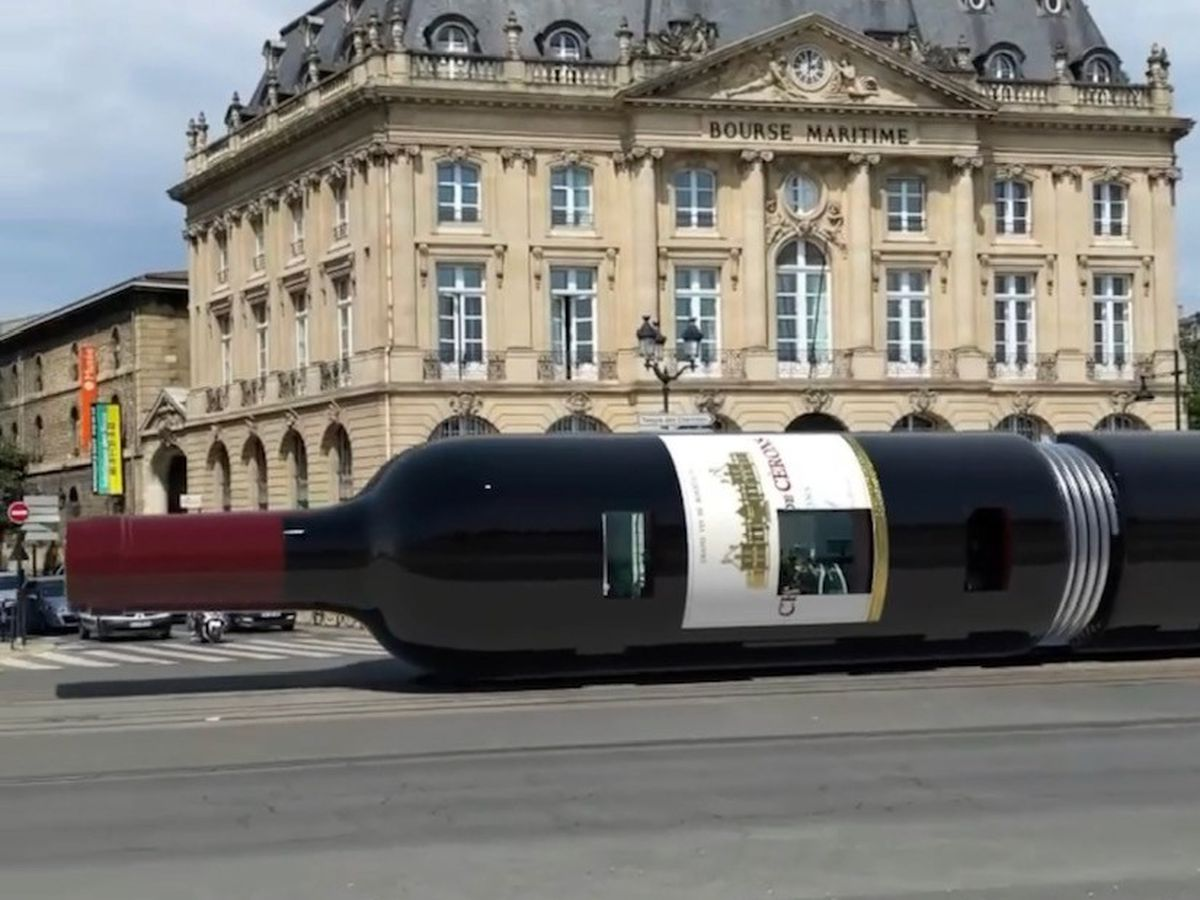
\includegraphics[scale=0.09]{Images/60c75cdf003a4_thumbnail_image0-5352442.jpg}}\\
	PhD on locality-aware scheduling of tasks sharing data on GPUs
	\begin{figure}[tb]
		\definecolor{green}{RGB}{70, 220, 70}
		\definecolor{orangegray}{RGB}{245, 191, 169}
		\centering
		\scalebox{0.5}{
		\begin{tikzpicture}[thick]
			\def\x{1.2}
			\def\y{1.5}
			\draw[color=black, fill=orangegray] (0*\x, 2*\y) rectangle (2*\x, 3*\y)  node[midway] {$\GPU{1}$ memory}; 
			\draw[color=black, fill=orangegray] (3*\x, 2*\y) rectangle (5*\x, 3*\y)  node[midway] {$\GPU{2}$ memory}; 
			\draw[color=black, fill=orangegray] (6*\x, 2*\y) rectangle (8*\x, 3*\y)  node[midway] {$\GPU{3}$ memory}; 
			\draw[color=black, fill=orangegray] (9*\x, 2*\y) rectangle (11*\x, 3*\y)  node[midway] {$\GPU{4}$ memory};
			\draw[color=black, fill=green] (0*\x, 0*\y) rectangle (11*\x, 1*\y) node[midway] {CPU memory of infinite size}; 
			\path[ultra thick] (5.5*\x,1*\y) edge (5.5*\x,1.4*\y); 
			\path[ultra thick] (1*\x,1.4*\y) edge node[midway, above] {PCI Express bus} (10*\x,1.4*\y); 
			\path[ultra thick] (1*\x,1.4*\y) edge (1*\x,2*\y); 
			\path[ultra thick] (4*\x,1.4*\y) edge (4*\x,2*\y);
			\path[ultra thick] (7*\x,1.4*\y) edge (7*\x,2*\y); 
			\path[ultra thick] (10*\x,1.4*\y) edge (10*\x,2*\y); 
			% Arrow 1
			\node at (-0.4, 0) (n1){};
			\node(n2)[above=3.5cm of n1]{};
			% this path will place/draw a node call (text)
			\scalebox{1.3}{\path (n1) -- node[sloped] (text) {Loading data} (n2);
			% Now draw arrows. This way it will be like you want.
			\draw[ultra thick][->] (n1)--(text)--(n2);}
			% Arrow 2
			\node at (10.5, 0) (n1){};
			\node(n2)[above=3.5cm of n1]{};
			\scalebox{1.3}{\path (n1) -- node[sloped] (text) {Evicting data} (n2);
			\draw[ultra thick][->] (n2)--(text)--(n1);}
		\end{tikzpicture}
		}
		\label{fig.topo}
	\end{figure}

\end{frame}
\nologo{
%% ---------------------------------------------------------------------------
\section{Motivation}
\begin{frame}{Motivation}
	\begin{block}{}
		\begin{itemize}
			\item Users may submits tens of hundreds of separate jobs using the same large input files
			\item Jobs will read inputs directly from a shared file system
			\item Large files increase the queue times of the next jobs on the node
		\end{itemize}
	\end{block}
	\successbox{\textbf{How can we minimize the amount of transfers between the shared file system and the nodes ?}}

	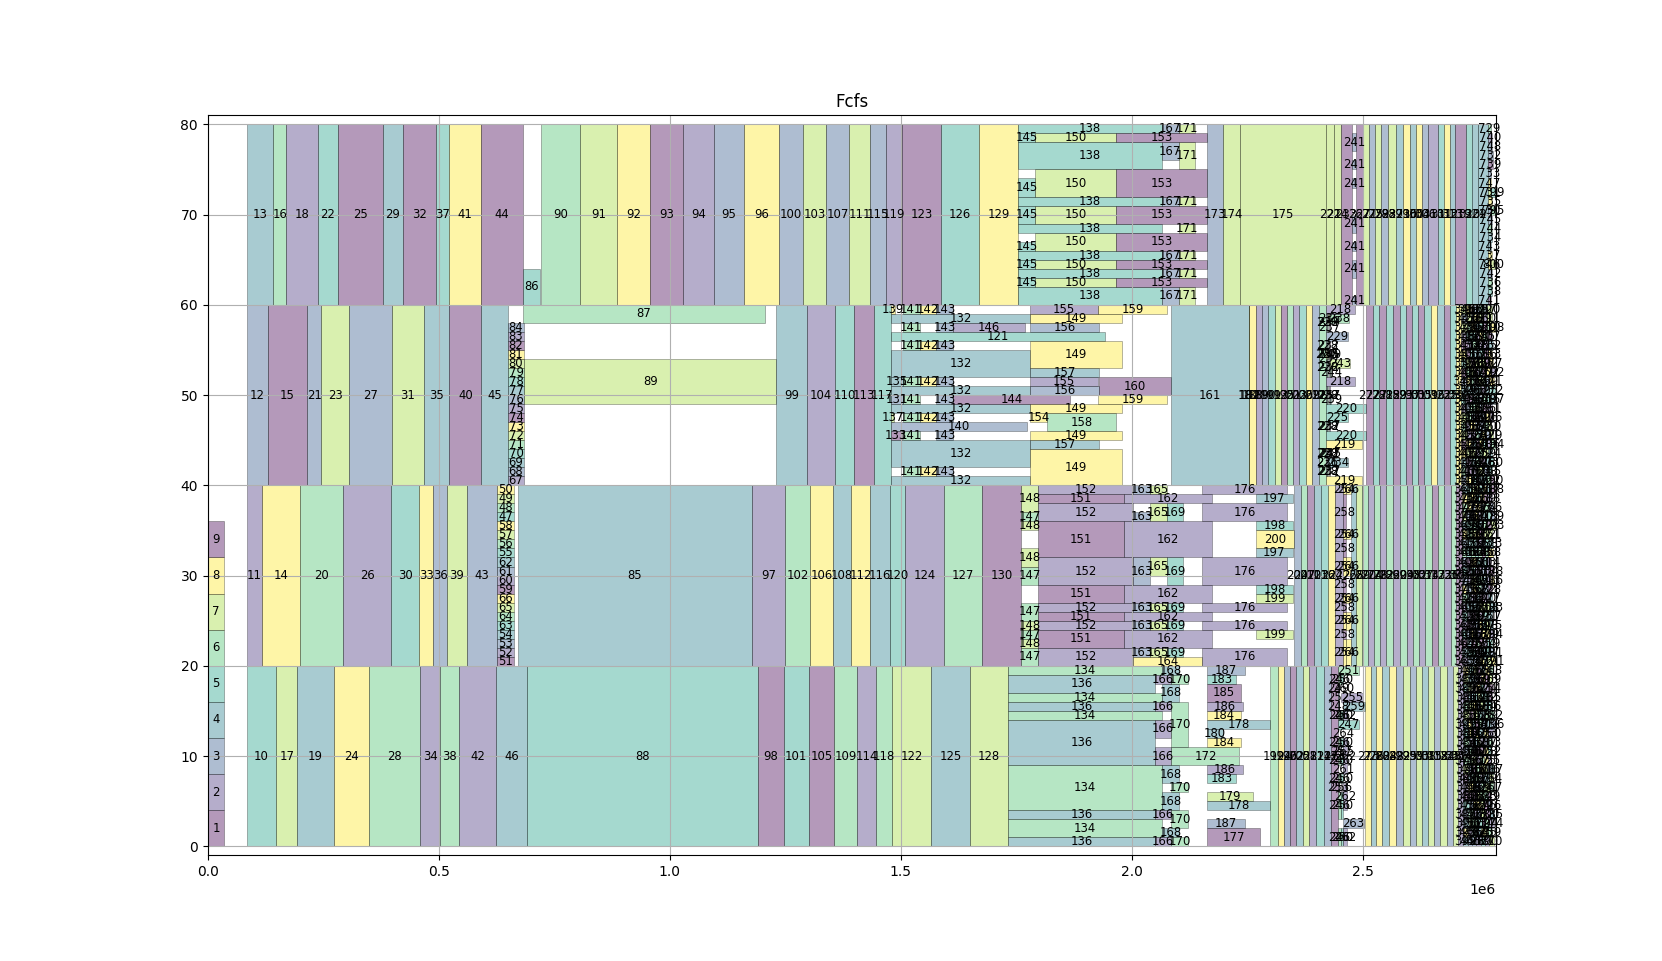
\includegraphics[scale=1]{../MBSS/plot/Gantt_charts/Fcfs800.png}
\end{frame}

%~ Fcfs800.png

%% ---------------------------------------------------------------------------
\section{Framework}
\begin{frame}{Framework}
	\begin{block}{Jobset \jobset}
		\begin{itemize}
			\item Set of jobs from Rackham's history with an added input file
			\item A file is shared by consecutive jobs submitted by the same user
			\item Each job require only one node and between $1$ and $20$ cores.
		\end{itemize}
	\end{block}
	\begin{block}{Nodes}
		\begin{itemize}
			\item Rackham's cluster (128, 256 and 1024 GB nodes)
			\item A file of size 1024 GB can only be scheduled on 1024 GB nodes
			\item Bandwidth of 0.1 GB/s for each node
			\item Each node has $N = 20$ cores
		\end{itemize}
	\end{block}
\end{frame}


%% ---------------------------------------------------------------------------
\subsection{Two different constraints}
\begin{frame}{Two different constraints}

\begin{block}{\bf Constraint 1: Dealing with file re-use}
	Maximize file re-use
\end{block}

\begin{block}{\bf Constraint 2: Dealing with different input files sizes}
	Allow smaller jobs to be computed on bigger nodes
\end{block}

		We define the \flow{J_i} of a job as:
		$$
			\flow{J_i} = \completiontime(J_i) - \submissiontime(J_i)
			\textbf{Obj.}: \quad \mathit{minimize}~\sum_{i=0}^{|\jobset|}\flow{J_i}
		$$
		\textbf{Objective: Minimize the mean \flow{} stretch}
		$$
			\textbf{Obj.}: \quad \mathit{minimize}~\frac{\sum_{i=0}^{|\jobset|}\frac{\flow{J_i}}{\duration(J_i) + \frac{\memory(\inputs(J_i))}{\bandwidth}}}{|\jobset|}
		$$
A secondary objective is to minimize the amount of file load.


\end{frame}

%% ---------------------------------------------------------------------------
\section{Algorithms}
%~ \begin{frame}{Algorithms}
%~ \begin{block}{2 schedulers from $\starpu$}
	%~ \begin{itemize}
		%~ \item EAGER (our baseline)
		%~ \item Deque Model Data Aware Ready (DMDAR)
	%~ \end{itemize}
%~ \end{block}
%~ \begin{block}{1 algorithm adapted from the literature}
	%~ \begin{itemize}
		%~ \item hMETIS
	%~ \end{itemize}
%~ \end{block}
%~ \begin{block}{Novel algorithm}
	%~ \begin{itemize}
		%~ \item Data-Aware Reactive Task Scheduling (DARTS)
	%~ \end{itemize}
%~ \end{block}
%~ \end{frame}

\begin{frame}{FCFS with a score}
	\begin{block}{2 schedulers from $\starpu$}
		
	\end{block}
\end{frame}

%% ---------------------------------------------------------------------------
\section{Experimental evaluation}
\subsection{Experimental settings}
\begin{frame}{Experimental settings}
        \begin{block}{General}
            \begin{itemize}
				\item Reduced cluster and set of jobs
				\item Get a set of jobs from Rackham's history and compute the starting state the day before the day we want to evaluate.
			\end{itemize}
        \end{block}
        \begin{block}{Evaluate file sharing}
            \begin{itemize}
				\item Each jobs is using a file
			\end{itemize}
		\end{block}
			\begin{block}{Evaluate size constraints}
			\begin{itemize}
				\item Tiled Cholesky decomposition (without dependencies) ($A = L \times L^T$)
			\end{itemize}
			\end{block}
\end{frame}

\begin{frame}{Flow stretch of FCFS with a score compared to FCFS on the file sharing constraint}
	\center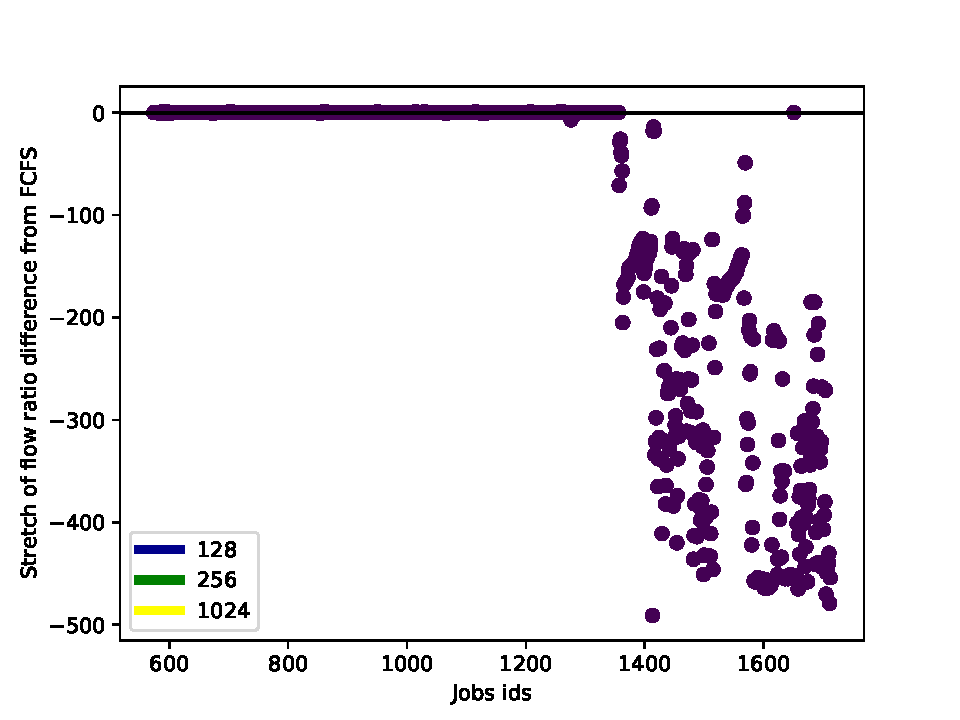
\includegraphics[scale=0.6]{../MBSS/plot/2022-02-08->2022-02-08_very_reduced_95_128_4_256_1_1024_FCFS_Score_x10_x7000_x0VSFCFS_stretch.pdf}
\end{frame}
\begin{frame}{Queue times of FCFS with a score compared to FCFS on the file sharing constraint}
	\center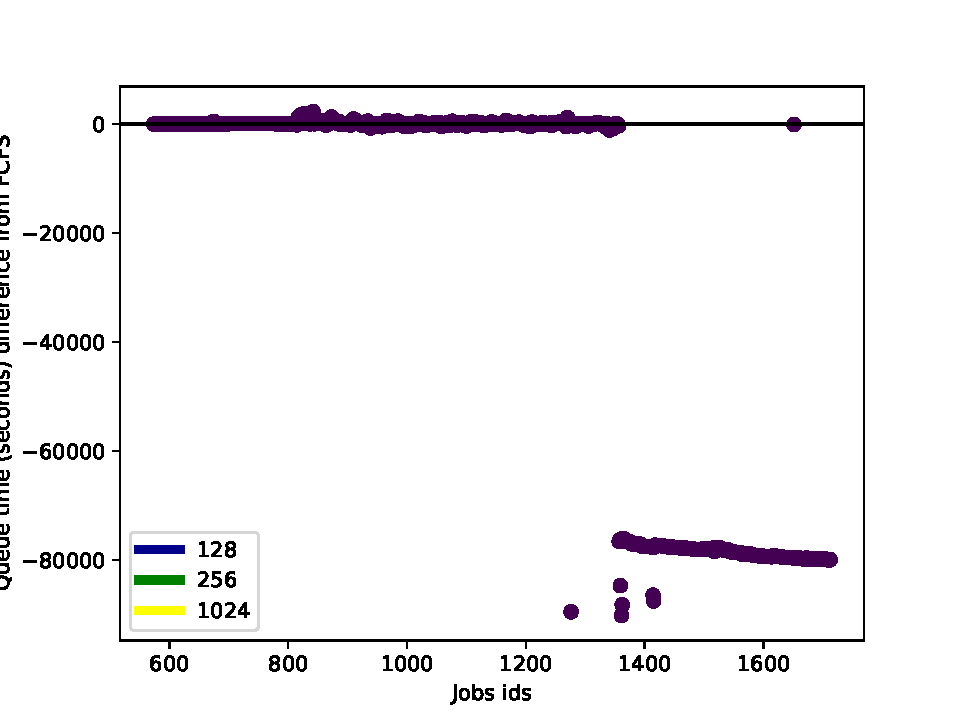
\includegraphics[scale=0.6]{../MBSS/plot/2022-02-08->2022-02-08_very_reduced_95_128_4_256_1_1024_FCFS_Score_x10_x7000_x0VSFCFS.pdf}
\end{frame}
\begin{frame}{Total Flow on the size constraint}
	\center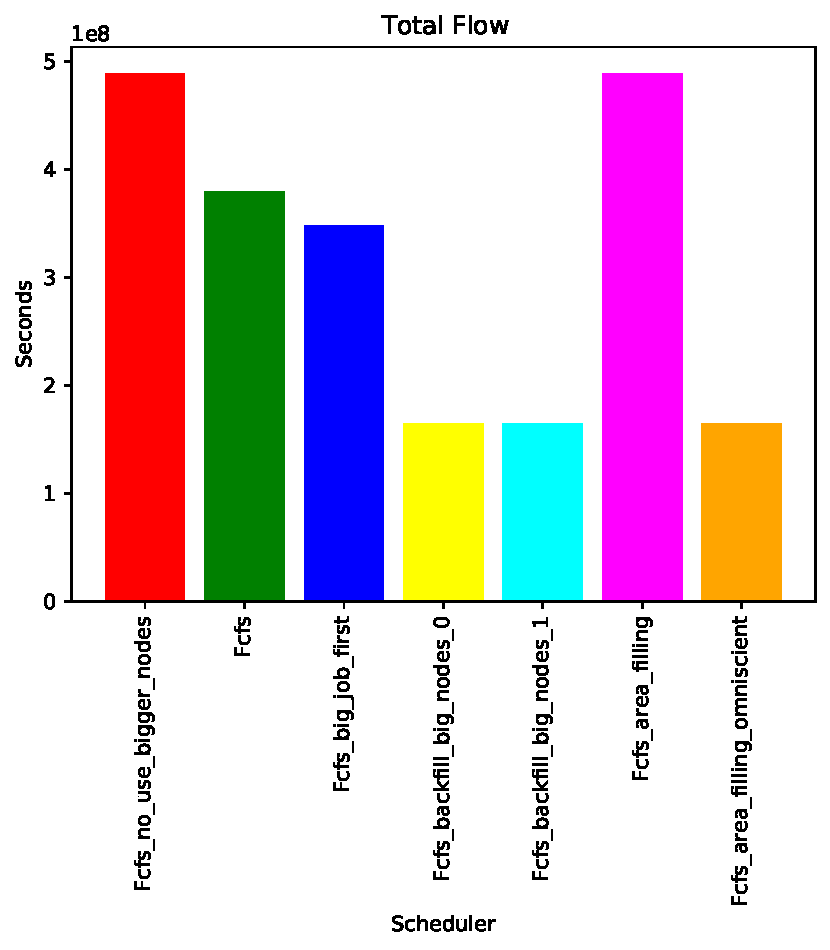
\includegraphics[scale=0.48]{../MBSS/plot/Size_Constraint_2022-02-08->2022-02-08_very_reduced_Total_flow_95_128_4_256_1_1024.pdf}
\end{frame}


%% ---------------------------------------------------------------------------
\section{Conclusion and future work}
\begin{frame}{Conclusion and future work}
\begin{block}{Limiting data movements is crucial to extract the most out of GPUs}
	Our contribution \MVRightarrow{}
	\emph{DARTS+LUF, focused on data locality}
\end{block}
%~ \begin{exampleblock}{Str}
		%~ \begin{itemize}
			%~ \item \textbf{Limits data transfers} thanks to the finding of an optimal data and an adapted eviction policy 
			%~ \item \textbf{Overlaps} communication and computations by distributing transfers over time
			%~ \item Can be used with a \textbf{reduced complexity}
		%~ \end{itemize}
%~ \end{exampleblock}		
	\begin{exampleblock}{Future work}
		\begin{itemize}
		\item Combine the 2 constraints
		\item Add backfilling
		\item Compare against FCFS EASY Backfilling
		\item Reduce complexity to test on full scale workloads and cluster
		\item Try implementation on SLURM ?
		\end{itemize}
	\end{exampleblock}
\end{frame}

}
\end{document}
